%-------------------------
% Resume in Latex
% Author 1chooo
% License : MIT
%------------------------

%---- Required Packages and Functions ----

\documentclass[a4paper,11pt]{article}
\usepackage{latexsym}
\usepackage{xcolor}
\usepackage{float}
\usepackage{ragged2e}
\usepackage[empty]{fullpage}
\usepackage{wrapfig}
\usepackage{lipsum}
\usepackage{tabularx}
\usepackage{titlesec}
\usepackage{geometry}
\usepackage{marvosym}
\usepackage{verbatim}
\usepackage{enumitem}
\usepackage[hidelinks]{hyperref}
\usepackage{fancyhdr}
\usepackage{fontawesome5}
\usepackage{multicol}
\usepackage{graphicx}
\usepackage{cfr-lm}
\usepackage[T1]{fontenc}
\setlength{\multicolsep}{0pt} 
\pagestyle{fancy}
\fancyhf{} % clear all header and footer fields
\fancyfoot{}
\renewcommand{\headrulewidth}{0pt}
\renewcommand{\footrulewidth}{0pt}
\geometry{left=1.4cm, top=0.8cm, right=1.2cm, bottom=1cm}
% Adjust margins
%\addtolength{\oddsidemargin}{-0.5in}
%\addtolength{\evensidemargin}{-0.5in}
%\addtolength{\textwidth}{1in}
\usepackage[most]{tcolorbox}
\tcbset{
	frame code={}
	center title,
	left=0pt,
	right=0pt,
	top=0pt,
	bottom=0pt,
	colback=gray!20,
	colframe=white,
	width=\dimexpr\textwidth\relax,
	enlarge left by=-2mm,
	boxsep=4pt,
	arc=0pt,outer arc=0pt,
}

\urlstyle{same}

\raggedright
\setlength{\tabcolsep}{0in}

% Sections formatting
\titleformat{\section}{
  \vspace{-4pt}\scshape\raggedright\large
}{}{0em}{}[\color{black}\titlerule \vspace{-7pt}]

%-------------------------
% Custom commands
\newcommand{\resumeItem}[2]{
  \item{
    \textbf{#1}{\hspace{0.5mm}#2 \vspace{-0.5mm}}
  }
}

\newcommand{\resumePOR}[3]{
\vspace{0.5mm}\item
    \begin{tabular*}{0.97\textwidth}[t]{l@{\extracolsep{\fill}}r}
        \textbf{#1}\hspace{0.3mm}#2 & \textit{\small{#3}} 
    \end{tabular*}
    \vspace{-2mm}
}

\newcommand{\resumeSubheading}[4]{
\vspace{0.5mm}\item
    \begin{tabular*}{0.98\textwidth}[t]{l@{\extracolsep{\fill}}r}
        \textbf{#1} & \textit{\footnotesize{#4}} \\
        \textit{\footnotesize{#3}} &  \footnotesize{#2}\\
    \end{tabular*}
    \vspace{-2.4mm}
}

\newcommand{\resumeProject}[4]{
\vspace{0.5mm}\item
    \begin{tabular*}{0.98\textwidth}[t]{l@{\extracolsep{\fill}}r}
        \textbf{#1} & \textit{\footnotesize{#3}} \\
        \footnotesize{\textit{#2}} & \footnotesize{#4}
    \end{tabular*}
    \vspace{-2.4mm}
}

\newcommand{\resumeSubItem}[2]{\resumeItem{#1}{#2}\vspace{-4pt}}

% \renewcommand{\labelitemii}{$\circ$}
\renewcommand{\labelitemi}{$\vcenter{\hbox{\tiny$\bullet$}}$}

\newcommand{\resumeSubHeadingListStart}{\begin{itemize}[leftmargin=*,labelsep=0mm]}
\newcommand{\resumeHeadingSkillStart}{\begin{itemize}[leftmargin=*,itemsep=1.7mm, rightmargin=2ex]}
\newcommand{\resumeItemListStart}{\begin{justify}\begin{itemize}[leftmargin=3ex, rightmargin=2ex, noitemsep,labelsep=1.2mm,itemsep=0mm]\small}

\newcommand{\resumeSubHeadingListEnd}{\end{itemize}\vspace{2mm}}
\newcommand{\resumeHeadingSkillEnd}{\end{itemize}\vspace{-2mm}}
\newcommand{\resumeItemListEnd}{\end{itemize}\end{justify}\vspace{-2mm}}
\newcommand{\cvsection}[1]{%
\vspace{2mm}
\begin{tcolorbox}
    \textbf{\large #1}
\end{tcolorbox}
    \vspace{-4mm}
}

\newcolumntype{L}{>{\raggedright\arraybackslash}X}%
\newcolumntype{R}{>{\raggedleft\arraybackslash}X}%
\newcolumntype{C}{>{\centering\arraybackslash}X}%
%---- End of Packages and Functions ------

%-------------------------------------------
%%%%%%  CV STARTS HERE  %%%%%%%%%%%
%%%%%% DEFINE ELEMENTS HERE %%%%%%%
\newcommand{\name}{Hugo ChunHo Lin} % Your Name
\newcommand{\course}{Dept. of Atmospheric Science, NCU.} % Your Program
\newcommand{\roll}{xxxxxxx} % Your Roll No.
\newcommand{\phone}{909-001068} % Your Phone Number
\newcommand{\emaila}{hugo970217@gmail.com} %Email 1
\newcommand{\emailb}{lcho0127@g.ncu.edu.tw} %Email 2
\newcommand{\myScore}{}
% \newcommand{\myScore}{GPA: 3.01/4.30; Rank: 25/33}




\begin{document}
\fontfamily{cmr}\selectfont
%----------HEADING-----------------


\parbox{2.35cm}{%
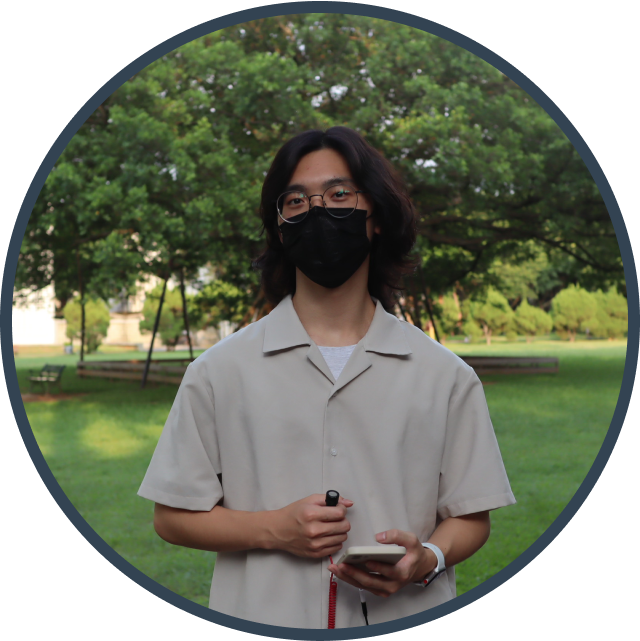
\includegraphics[width=2cm,clip]{1chooo.png}
}
\parbox{\dimexpr\linewidth-2.8cm\relax}{
\begin{tabularx}{\linewidth}{L r} \\
  \textbf{\Large \name} & {\raisebox{0.0\height}{\footnotesize \faPhone}\ +886-\phone}\\
  XinYi, Taipei, Taiwan. & \href{mailto:\emaila}{\raisebox{0.0\height}{\footnotesize \faEnvelope}\ {\emaila}} \\
  Major: \course &  \href{mailto:\emailb}{\raisebox{0.0\height}{\footnotesize \faEnvelope}\ {\emailb}}\\
  {Minor Specialty: Dept. of CSIE, NCU.} &  \href{https://github.com/1chooo}{\raisebox{0.0\height}{\footnotesize \faGithub}\ {1chooo}} \\
  {Program: Interdisciplinary AI Program, NCU.} & \href{https://www.linkedin.com/in/1chooo/}{\raisebox{0.0\height}{\footnotesize \faLinkedin}\ {Hugo ChunHo Lin}}
\end{tabularx}
}
% \parbox{3.0cm}{%
% \flushright 
\includegraphics[width=2cm,clip]{nitp_logo.png}
% }




%-----------EDUCATION-----------
% \section{\textbf{Education}}
%   \resumeSubHeadingListStart
%     \resumeSubheading
%       {National Central University (NCU)}{3.01/4.30 - 25/33}
%       {BS, Department of Atmospheric Science}{Sep. 2020 - Jun. 2024}
%       \resumeSubheading
%       {National Central University (NCU)}{}
%       {Specialty Minor, Department of Computer Science \& Information Engineering}{Sep. 2021 - Jun. 2024}
%       \resumeSubheading
%       {National Central University (NCU)}{}
%       {Program, AI Cross-domain Program}{Sep. 2021 - Jun. 2024}
%   \resumeSubHeadingListEnd
  
% \vspace{-5.5mm}
%

%-----------EDUCATION TEST-----------------
\section{\textbf{Education}}
  \resumeSubHeadingListStart
    \resumeSubheading
      {National Central University}{\myScore}
      {Bachelor scholarship}{Sep. 2020 - present}
      \vspace{-1.0mm}
      \resumeItemListStart
        \item {Mater: Department of Atmospheric Science}
        \item {Specialty Minor: Department of Computer Science \& Information Engineering}
        \item {Program: Interdisciplinary AI Program}
      \resumeItemListEnd      
  \resumeSubHeadingListEnd
\vspace{-8.5mm}


%-----------EXPERIENCE-----------------
\section{\textbf{Work Experience}}
  \resumeSubHeadingListStart
    \resumeSubheading
    {Teaching Assistant}{}
    {Teaching Assistant in the course "Freshman English", NCU.}{Aug. 2022 - present}
    \vspace{-2.0mm}
    \resumeItemListStart
    % \item {Work description line 1}
    % \item {Work description line 2}
    \resumeItemListEnd
    
    \vspace{-3.0mm}

    \resumeSubheading
      {Website Administrator}{}
      {Manage the data in website, server maintenance, the center for Teaching Education, NCU.}{July. 2022 - Jan. 2023}
      \vspace{-2.0mm}
      \resumeItemListStart
    \item {Manage website data and maintain the server.}
    \item {Launch a project aimed at developing a system to manage and track student progress.}
    \resumeItemListEnd
    
    \vspace{-3.0mm}
    
    
    \resumeSubheading
      {Teaching Assistant}{}
      {Teaching Assistant in the course "Student Service-Learning", NCU.}{Feb. 2021 - Jun. 2021}
      \vspace{-2.0mm}
      \resumeItemListStart
    % \item {Work description line 1}
    % \item {Work description line 2}
    \resumeItemListEnd
      
  \resumeSubHeadingListEnd
\vspace{-8.5mm}

\section{\textbf{Extracurricular Activity}}
  \resumeSubHeadingListStart
    \resumeSubheading
      {{\href{https://ncufresh22tmp.le37.tw/blog/}{NCUFresh Team(NCUBlog)}}}{}
      {Website developer team for the incoming freshmen admitting to NCU.}{Dec. 2021 - Jul. 2022}
      \vspace{-1.0mm}
      \resumeItemListStart
        \item {The essential experience of manage larger projects with teammate.}
        \item {Frontend skills: UI/UX, Figma.}
        \item {Teamwork: leadership, meeting arrangement, facilitating communication, project demo.}
        \item {Marketing: increase social media reach, content of films and articles.}
      \resumeItemListEnd

    % \resumeSubheading
    % {Teaching Assistant}{}
    % {Teaching Assistant in the course "Freshman English", NCU.}{Aug. 2022 - present}
    % \vspace{-2.0mm}
    % \resumeItemListStart
    % % \item {Work description line 1}
    % % \item {Work description line 2}
    % \resumeItemListEnd
    
    \vspace{-3.0mm}
    
    
    \resumeSubheading
      {{\href{https://github.com/NCUAppTeam}{NCUAPP Team}}}{}
      {Make NCU better, NCU.}{Mar. 2023 - present}
      \vspace{-2.0mm}
      \resumeItemListStart
    % \item {Work description line 1}
    % \item {Work description line 2}
    \resumeItemListEnd
    \vspace{-3.0mm}
    
    
    \resumeSubheading
      {Co-captain(Basketball Team)}{}
      {Basketball Team Co-captain in my department, Dept. ATM, NCU.}{Aug. 2022 - present}
      \vspace{-2.0mm}
      \resumeItemListStart
    % \item {Work description line 1}
    % \item {Work description line 2}
    \resumeItemListEnd
      
  \resumeSubHeadingListEnd

      
      
  % \resumeSubHeadingListEnd
\vspace{-8.5mm}



%-----------PROJECTS-----------------
\section{\textbf{Projects(ML)}}
\resumeSubHeadingListStart

    \resumeProject
      {\href{https://github.com/1chooo/CNN-handwriting-detection}{CNN Handwriting Detection}} %Project Name
      {A CNN-driven method for detecting and classifying handwriting.} %Project Name, Location Name
      {Jun. 2022} %Event Dates

      \resumeItemListStart
        \item {The first project of neural network.}
        \item {Test Accuracy: Up to 97.12\%}
        \item {What I have done: Solve overfitting, practice building types of layer.}
    \resumeItemListEnd
    \vspace{-2mm}
    
    \resumeProject
      {\href{https://github.com/1chooo/rain_prediction}{Rainy Percentage Prediction}} %Project Name
      {ML-based estimation of the chance of rainfall.} %Project Name, Location Name
      {Jun. 2022} %Event Dates

      \resumeItemListStart
      \item {Combine the Atmospheric Science with AI(tradition v.s. technology).}
      \item {Exploring how the new capabilities of AI will change the future of rainfall prediction.}
      \item {What I have done: Data mining(20 yrs), model training, represent results on web(python flask).}
    \resumeItemListEnd
    \vspace{-2mm}

    % KAGGLE
    % \resumeProject
    %   {Kaggle Practice} %Project Name
    %   {Project description(Your input in the project)} %Project Name, Location Name
    %   {Jan. 2023} %Event Dates

    %   \resumeItemListStart
    %     \item {Tools \& technologies used: python, }
    %     \item {More description on the project(The output you achieved by working on the project)}
    % \resumeItemListEnd
    % \vspace{-2mm}
    
      
  \resumeSubHeadingListEnd
  \vspace{-5.5mm}

%-----------INTERESTS-----------------
\section{\textbf{Research Interests}}
  \resumeSubHeadingListStart
    \resumeSubheading
      {Computer Science}{}
      {OS, Programming Language, Algorithm, Parallel Computing.}{}
      \resumeSubheading
      {Atmospheric Science}{}
      {With ML method to improve Numerical Weather Prediction, automation in meteorology.}{}
      % \resumeSubheading
      % {National Central University (NCU)}{}
      % {Program, AI Cross-domain Program}{Sep. 2021 - Jun. 2024}
  \resumeSubHeadingListEnd
  
\vspace{-5.5mm}
% \section{\textbf{Interests}}
% \resumeSubHeadingListStart

%     \resumeProject
%       {\href{https://github.com/1chooo/CNN-handwriting-detection}{CNN Handwriting Detection}} %Project Name
%       {Project description(Your input in the project)} %Project Name, Location Name
%       {Jun. 2022} %Event Dates

%       \resumeItemListStart
%         \item {Tools \& technologies used: python, tensorflow, keras}
%         \item {More description on the project(The output you achieved by working on the project)}
%     \resumeItemListEnd
%     \vspace{-2mm}
    
%     \resumeProject
%       {Rainy Percentage Prediction} %Project Name
%       {Project description(Your input in the project)} %Project Name, Location Name
%       {Jun. 2022} %Event Dates

%       \resumeItemListStart
%         \item {Tools \& technologies used: python, }
%         \item {More description on the project(The output you achieved by working on the project)}
%     \resumeItemListEnd
%     \vspace{-2mm}

%     % KAGGLE
%     % \resumeProject
%     %   {Kaggle Practice} %Project Name
%     %   {Project description(Your input in the project)} %Project Name, Location Name
%     %   {Jan. 2023} %Event Dates

%     %   \resumeItemListStart
%     %     \item {Tools \& technologies used: python, }
%     %     \item {More description on the project(The output you achieved by working on the project)}
%     % \resumeItemListEnd
%     % \vspace{-2mm}
    
      
%   \resumeSubHeadingListEnd
%   \vspace{-5.5mm}
  
  
  
  %-----------Technical skills-----------------
  % \section{\textbf{Technical Skills and Interests}}
  \section{\textbf{Technical Skills}}
  \begin{itemize}[leftmargin=0.05in, label={}]
    \vspace{1.0mm}
    {\item{
      \textbf{Languages}{: Python, c/c++, Java, Assembly, JavaScripts, LaTeX, etc.} \\
      % \textbf{ML/DL}{: Linear Regression, Random Forest, Policy Gradient, CNN, DNN, etc.} \\
      \textbf{ML/DL}{: Keras, Tensorflow, Scikit-learn, Numpy, Pandas, etc.} \\
      \textbf{Developer Tools}{: VSCode, Vim, Pycharm, Jupyter notebook, etc.} \\
      % \textbf{Frameworks}{: } \\
      % \textbf{Operating System}{: Linux, MacOS, Windows.} \\
      \textbf{Cloud/Databases}{: Colab, AWS, mySQL.} \\
      \textbf{Soft Skills}{: Git, GUI, line bot, blog.} \\
      \textbf{Coursework}{: More Information on my \href{https://github.com/1chooo}{GitHub} or my \href{https://sites.google.com/g.ncu.edu.tw/1chooo}{Personal Website.}} \\
      % \textbf{Areas of Interest}{: Data Visualize, Data Mining, Algorithm, OS, Programming Language} \\
    }}
    % \small{\item{
    %  \textbf{Languages}{: python, c, cpp, java, assembly lang, JavaScripts, LaTeX, etc.} \\
    %  \textbf{Developer Tools}{: VSCode, Vim, Pycharm, CLion, IntelliJ, Colab, Jupyter Notebook} \\
    % %  \textbf{Frameworks}{: } \\
    %  \textbf{Cloud/Databases}{: AWS, sql, GCP} \\
    %  \textbf{Soft Skills}{: GUI, ChatGPT, StackOverflow, leadership, communication} \\
    %  \textbf{Coursework}{: CNN Handwriting Dection, Rain Prediction with ML, Kaggle Contest} \\
    %  \textbf{Areas of Interest}{: Data Visualize, Data Mining, Algorithm, OS, Programming Language} \\
    % }}
 \end{itemize}
 \vspace{-16pt}



% %-----------Positions of Responsibility-----------------
% \section{\textbf{Positions of Responsibility}}
% \vspace{-0.4mm}
% \resumeSubHeadingListStart
% \resumePOR{Position, } % Position
%     {Club or Event} %Club,Event
%     {Position tenure} %Tenure Period
% \resumePOR{Position, } % Position
%     {Club or Event} %Club,Event
%     {Position tenure} %Tenure Period
% \resumeSubHeadingListEnd
% \vspace{-5mm}




%-----------Achievements-----------------
% \section{\textbf{Achievements}}
% \vspace{-0.4mm}
% \resumeSubHeadingListStart
% \resumePOR{Achievement } % Award
%     {description} % Event
%     {Event dates} %Event Year
    
% \resumePOR{Achievement } % Award
%     {description} % Event
%     {Event dates} %Event Year
% \resumeSubHeadingListEnd
% \vspace{-5mm}



%-------------------------------------------
\end{document}
